\chapter{Problem Statement}
\label{cha:multiObjectiveOptimization}



%---------------------------------------------------------------------------

\section{Multi-Objective Optimization}
\label{sec:multi}

The main goal of optimization is to find the very best solution from a most likely infinite set of possibilities.
Optimization procedure relies on finding and comparing feasible solutions until no better solution can be found.
Each solution can be classified as good or bad in terms of a specific objective we are interested in.
E.g. we could define objective as the cost of fabrication, efficiency of a technological process, etc.
Contrary to single-objective optimization there is no clearly defined optimum, instead of that we have to deal with a set of trade-off optimal solutions.
They are generally known as Pareto-optimal solutions (\cite{Phd}).

Vast majority of real-world problems involve more than one objective.
That's why it is so crucial to develop methods to efficiently solve them.
(\cite{Phd}, \cite{Deb:2001:MOU:559152})

\subsection{Formal definition}

Multi-objective optimization problem (MOOP) deals with more than one objective function.
It turns out that objectives are most likely contradictory which makes the MOOP difficult to solve.
In fact it is the most common situation we will ever encounter. 
Following \cite{Deb:2001:MOU:559152} - formal definition of MOOP is being defined as follows:

\begin{equation} 
MOOP \equiv
 \begin{cases}
     Minimize/Maximize  & f_{m}(\bar{x}), \text{ } m = 1,2...,M \\
     Subject \text{ } to  &  g_{j}(\bar{x}) \geq 0, \text{ } j = 1,2..., J  \\ 
			  &  h_{k}(\bar{x}) = 0, k = 0,1...,K \\
			  &  x_{i}^{(L)} \leq x_{i} \leq x_{i}^{(U)}, i = 1,2...,N
      
\end{cases}  
\end{equation}

These constraints and bounds ($g_{j}(x) , h_{k}(x) $ are constraint functions and there are $M$ objective functions) constitute a \emph{decision space}. 
\cite{Deb:2001:MOU:559152}
Any solution that satisfies all the constraints and bounds is called a \emph{feasible solution} \cite{Deb:2001:MOU:559152}.

It turns out that the set of feasible solutions is partially ordered.
In order to compare two solutions we introduce \emph{Pareto dominance} relation \cite{Phd}:

\begin{equation}
\bar{x}_{A}  \prec \bar{x}_{B} \equiv
      \begin{cases}
     \exists{i \in 1..M} : f_{i}(\bar{x}_{A}) < f_{i}(\bar{x}_{B}) \\
     \neg (\exists{j \in 1..M} : f_{j}(\bar{x}_{A}) > f_{j}(\bar{x}_{B}))  \\ 
			  
      
\end{cases} 
\end{equation}

Solution that is not dominated by any other solution is called \emph{non-dominated}. 
The set of \emph{non-dominated} solutions is what we are actually trying to find while dealing with MOOPs.



\begin{figure}[H]
  \begin{center}
    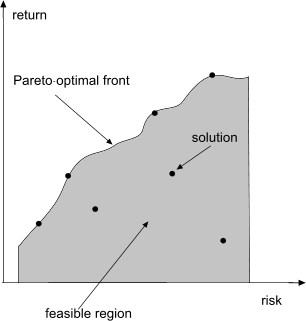
\includegraphics[scale=.9]{pareto_front.png}
  \end{center}
  \caption{Pareto-optimal front of portfolio optimization problem}
\end{figure}


Pareto-optimal front is the set of choices that are \emph{non-dominated} (\cite{Dre}).
 

\subsection{Portfolio Optimization Problem}

Portfolio optimization problem is an example of MOOP.
Portfolio is a set of assets or equities (e.g. stocks) owned by an investor.
Investors cannot rely solely on their intuition to make the right choice.
It is obvious that every investor would like to have the highest return possible.
Unfortunately, equities with high returns usually correlate with high risk. 
That is why it is up to the investor to decide what level of risk are acceptable.

%---------------------------------------------------------------------------

\section{Capital Asset Pricing Model}
\label{CAPM}

%\cite{CAPM}

Modern Portfolio Theory (MPT) (introduced by Harry Markowitz in 1952) was a tremendous breakthrough. 
Investors could finally use a mathemathical approach to construct their portfolios.
Most of them used solely diversification as a mean of reducing portfolio's risk.
With brand new theory they did not have to rely only on common sense - the investment risk was finally expressed in quantitative terms. 

Nevertheless MPT is not perfect, even its creators are fully aware that it has some very important limitations.
The following assumptions of MPT are responsible for its shortcomings [\cite{MPT}]:
\begin{itemize}
  \item variance of portfolio returns is the correct measure of investment risk
  \item investment returns of all assets can be adequately represented by the normal distribution
\end{itemize}

  

Capital Asset Pricing Model (CAPM) was developed in 1960s by Sharpe (\cite{CAPM-Sharpe}) and Lintner.
 
As well as MPT it tries to find the relationship between the price of a single asset and its risk.
Answering the question of how to calculate a risk as well as return of any asset being a part of portfolio is of paramount importance to each investor.

The Sharpe capital asset pricing model is based on the following assumptions \cite{CAPM}:

\begin{itemize}
  \item all investors are risk aversing
  \item all investors have the same information about the market
  \item capital markets are perfect - no transaction costs, no tax, all assets are infinitely divisible
  \item all investors view the expected returns and standard deviations of return provided by different portfolios in the same way
\end{itemize}
 
Lets assume that investor portfolio contains $N$ assets, then according to Capital Asset Pricing expected return of asset $i$ is \cite{CAPM}: 

\begin{equation}
\label{first_eq}
 E(R_{i})  = R_{f} + \frac{ [E(R_{m}) - R_{f}]} {\sigma^2(R_{m})} cov(R_{i}, R_{m})
\end{equation} 

\begin{description}
  \item [$E(R_{i})$]
    expected return of asset $i$
  \item [$R_{f}$]
    risk-free rate of interest (e.g. government bonds)
  \item [$E(R_{m})$]
    expected return of the market
  \item [$\sigma^2(R_{m})$]
    variance of the market return
  \item [$cov(R_{i}, R_{m})$]
    covariance between market return and asset $i$ return
\end{description}

While the risk associated with entire portfolio is equal to:

\begin{equation}
\label{sec_eq}
 \sigma_{p}  = \sqrt{\sum_{i} \sum_{j} w_{i}w_{j} \sigma_{i} \sigma_{j} \rho_{ij}}
\end{equation} 

\begin{description}
  \item [$\sigma_{p}$]
    portfolio risk
  \item [$w_{i}$]
    weighting of component asset $i$
  \item [$w_{j}$]
    weighting of component asset $j$
  \item [$\sigma_{i}$]
    standard deviation of asset $i$
  \item [$\sigma_{j}$]
    standard deviation of asset $j$
  \item [$\rho_{ij}$]
    correlation coefficient between the returns on assets $i$ and $j$
\end{description}
 
%---------------------------------------------------------------------------

\section{Trend following}
\label{sec:trendFollowing}

\subsection{Trend following fundamentals}
\label{sec:trend_following_fundamentals}

The concept of price as the trading cue lays the foundations for trend following (TF). 
Contrary to other trading strategies based on fundamental analysis (which use factors like: overall state of the economy, interest rates, production, etc. to predict stock price)
TF use only price as the key trading variable. 

Trend following basically does not try to predict when the trend will occur. 
Instead of that, trend followers will react to the market's movement and adapt accordingly.
This strategy simply analyses stock prices and decides whether the current situation is suitable for buying or selling a specific stock.
Market breakouts are a great buying opportunities, when you recognize that you are wrong you exit immediately in order to cut losses.
Set of predefined rules decides  whether to take any action (they should recognize when the trend starts as well as when to exit) so the entire process can be easily automated.
Such rules are quite simple but disciplined execution of them could lead to achieving spectacular returns year after year.
It is all about cutting the losses and letting the profits run.
Many leading hedge funds successfully use strategies based on trend following to manage their portfolios. (\cite{Trend01})  

\begin{figure}[H]
  \begin{center}
    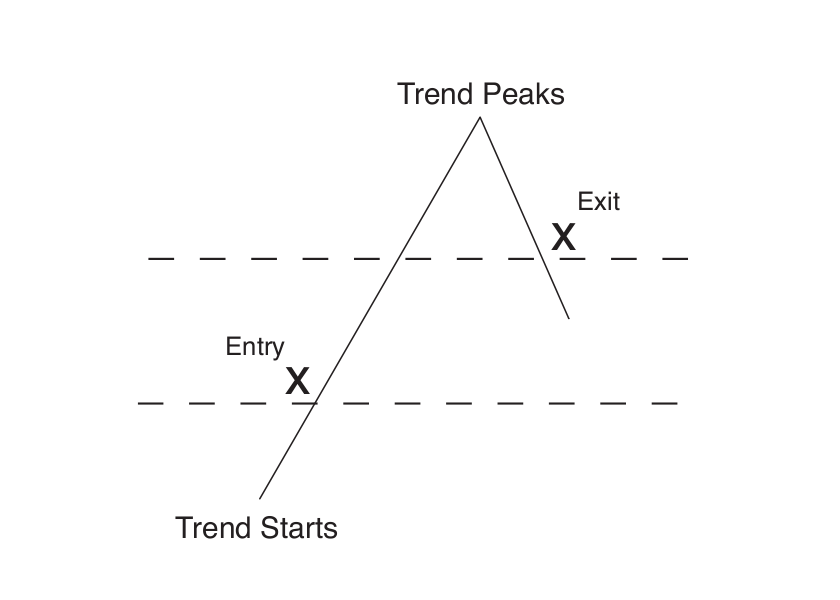
\includegraphics[scale=.4]{trend_following.png}
  \end{center}
  \caption{Simple example of how trend following works in practise}
\end{figure}

Another advantage of this investing method is the fact that investor does not have to know much about what is being traded (it could be stocks, oil, gold, etc.).
Normally, people tend to gather some information about the company they are willing to invest in. 
They analyse its market situation, competitors, financial performance, etc. which is time consuming, especially for someone who is not a professional trader.
With trend following we just have to to focus on elaborating trading rules that should reflect our trading strategy.
After that we can automate the decision making process by designing and implementing our own trading system.   

\subsection{Types of trends}

There are three main types of trends:

\begin{description}
  \item [short-term trend]
      Any price movement that occurs over a few hours or days.
  \item [intermediate-term trend]
      General movement in price data that lasts from three weeks to six months.
  \item [long-term trend]
      Any price movement that occurs over a significant period of time, often over one year or several years.
\end{description}



\subsection{Designing trading system based on trend following} 

Following \cite{Trend01}, the core of each trading system based on trend following strategy is a set of rules governing each buy/sell decision.
More specifically we have to devise rules to answer the following questions:

\begin{itemize}
  \item how much money are we willing to put on a single trade
  \item when to exit (what kind of losses are acceptable)
  \item when to enter (when the trend has started) 
  \item what markets are we interested in and how to split money between them (we would like to have a diverse portfolio (stocks, gold, etc.))
\end{itemize}

These rules should reflect our investing style.

In \ref{trend_following_impl} a system based on trend following strategy is presented in more details.

%---------------------------------------------------------------------------

\section{Evolutionary Algorithms}
\label{sec:evolAlgorithms}

Each stochastic optimization method based on a simulation of evolution process (natural evolution is simulated by an iterative computation process)
can be termed as the Evolutionary Algorithm (EA).
Most commonly known examples of EA include genetic algorithms and evolutionary programming.
A set of candidate solutions, which is modified by the principles of evolution (selection and variation), is used by all above approaches.
Some of solutions present in the population set are better than others (we can assign a fitness value to each solution).
The fitter the solution the more likely it will reproduce.
By means of recombination and mutation new chromosomes are introduced into existing population.
Despite the fact that the principles are quite simple, the resulting algorithm is a powerful search mechanism.  

Apart from all advantages mentioned above, evolutionary algorithms are especially usefull to solve \emph{Multi Objective Optimization Problems} because they
can find multiple \emph{non-dominated} solutions at once. 
According to some researchers evolutionary algorithms are much better suited for MOOPs than strategies based on blind search \cite{Phd}.

\subsection{Basic Principles of Evolutionary Algorithms}

Following \cite{Phd}, EA can be characterized by:

\begin{itemize}
  \item set of possible solutions is kept throughout the algorithm execution
  \item selection process (low quality individuals are removed while well fitted are allowed to reproduce)
  \item set of possible solutions is manipulated by genetic operators (e.g. mutation and recombination)
\end{itemize}

Solution candidates are usually called \emph{individuals} and the entire set of them is called a \emph{population}. 
   
\section{Co-evolutionary Algorithms}
\label{sec:co-evol}

Co-evolutionary algorithms rely on process of co-evolution (two or more species coexist and interact in the same environment).
Individuals of one species interact with each other as well as with members of other species (which simulates the process of adaptation of different species cohabitating the same 
ecosystem).
  
Following \cite{Dre}, co-evolutionary interactions could include:

\begin{itemize}
  \item competition for limited resources
  \item predator-prey interactions
  \item host-parasite interactions
  \item mutualism
  \item commensalism
\end{itemize}

The fitness of each individual simultaneously depends on fitness of the solution as well as other individuals' quality.
The biggest advantage of co-evolutionary algorithms is their ability to maintain population diversity which is crucial to obtain many good solutions in a single algorithm run.    

  

%-------------------------------------------------------------------------------------------------

\section{Genetic Algorithms}
\label{sec:genAlgorithms}

Many computational problems require searching through a huge search space.
Such problems can substantially benefit from an effective use of parallelism.
In that case, many different possibilities are explored simultaneously. 
It turns out that the process of biological evolution could provide an efficient method for addressing these problems.(\cite{Mitchell01})
Because of this genetic algorithms belong to a class of Evolutionary Algorithms (\ref{sec:evolAlgorithms}).


The principles of genetics and natural selection lay the foundations for genetic algorithms (GAs).
GAs are very powerfull tool to solve search and optimization problems.

GAs rely on an evolving population composed of many individuals trying to maximize their \emph{fitness} (i.e., maximizes the return, minimizes cost of fabrication).  
The method was developed by John Holland (1975) over the course of the 1960s and 1970s.(\cite{Haupt:2004:PGA:1007746})

\subsection{Elements of genetic algorithms}

Almost all genetic algorithms have some elements in common \cite{Mitchell01}:
\begin{itemize}
  \item populations of chromosomes
  \item selection according to fitness
  \item crossover to produce new offspring
  \item random mutation of new offspring
  \item fitness function
\end{itemize}

\begin{figure}[H]
  \begin{center}
    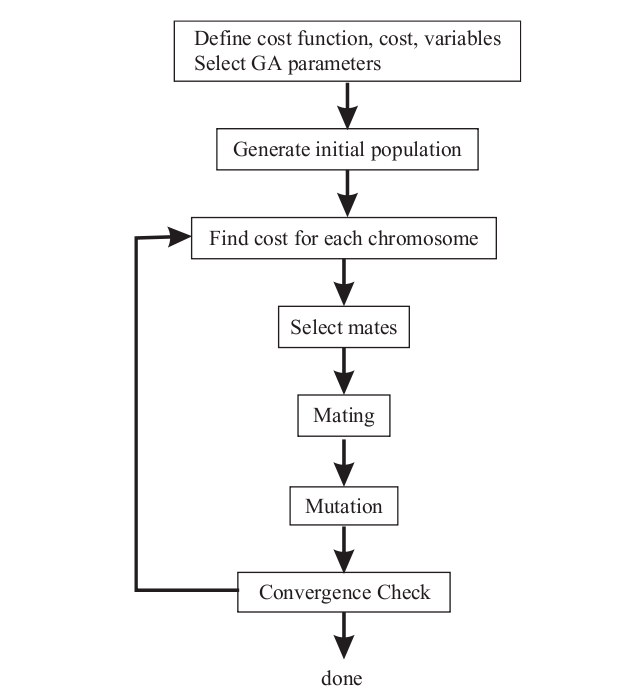
\includegraphics[scale=.4]{GA_flow.png}
  \end{center}
  \caption{GA flow chart \cite{Haupt:2004:PGA:1007746}}
\end{figure}

The GA operates on populations of chromosomes, successively changing one such population to another (by using GA operators: mutation, selection, crossover, etc.). 
Each chromosome contains potential solution to a problem (e.g. represented as binary string). 
Fitness functions are used to assess how well specific chromosome solves the problem.
The better fitting chromosomes are more likely to be involved in reproduction process.
That mimics the biological process of evolution - fitness of an organism is obtained by means of random variation (mutation, recombination, etc.) and natural selection
thus propagating genetic material to future generations.
These rules seems to be simple but they are in fact responsible for extraordinary variety and complexity of the biosphere.
\cite{Mitchell01} 
 
According to \cite{Mitchell01} , high parallelism, discovering and emphasizing solutions that are already quite good are the main reason why GAs work.  
 

\subsection{Genetic algorithms operators}

Following \cite{Mitchell01} - the simplest form of genetic algorithm involves three types of operators: selection, crossover and mutation. 

\begin{description}

\item[selection]
  This operator is responsible for selecting chromosomes from the population for reproduction.
  Likelihood of being chosen is based on the value of fitness function (the fitter the chromosome the better).
  
\item[crossover]
  The crossover operator is responsible for exchanging genetic material between chromosomes.
  Implemantation involves cutting points selection and then cut parts of chromosomes are exchanged.

\item[mutation]
  This operator introduces random changes to a chromosome.
  The probability of random change introduction is usually very small.  

\end{description}

%---------------------------------------------------------------------------

\section{Multiagent Systems}
\label{sec:multi}

There is no universally accepted definition of the term \emph{agent}.
Nevertheless majority of researchers agree that \emph{agent} operates inside some \emph{environment} and should be capable of \emph{autonomous action}.
There is little agreement beyond this. (\cite{Weiss}) 
 
In theory it is possible to imagine a single agent working in an environment but it is quite rare.
The most common situation is a group of autonomous agents interacting inside the environment.
In order to be capable of fulfilling all the above requirements environments have to provide means of communications and interactions to all agents within.

\subsection{Intelligent agents}

The most usefull type of \emph{agents} is called \emph{intelligent agent}.
The \emph{intelligent agent} is capable of (\cite{Weiss}):

\begin{description}
  \item [reactivity]
	  agents can respond to changes in the environment and properly adjust to new conditions
  \item [pro-activeness]
	  agents take the initiative to accomplish their goals
  \item [social ability]
	  agents are capable of intelligent interaction with other agents to satisfy their objectives
\end{description}

\subsection{Co-evolutionary Multi-agent System (CoEMAS)}
\label{sec:CoEMAS}

According to  \cite{Dre} ,\cite{Dre2}, CoEMAS contains the following elements:

\begin{itemize}
  \item the environment 
  \item the set of species that co-evolve 
  \item the set of different resource types (there should be at least one resource type)
\end{itemize}

  
Additionally we define the set of actions that agent can perform :

\begin{description}
  \item [die]
      agent dies when the amount of resources it helds is too low to sustain life (freed resource is given back to environment)
  \item [accept]
      agent accepts partner for reproduction (only agents having more than threshold amount of resources are taken into account)
  \item [give]
      agent is obliged to give some resource to other agent
  \item [get]
      agent is allowed to get some resource from other agent
  \item [seek]
      agent finds another agent so actions like get and finding appropriate partner for reproduction can be perform
  \item [clone]
      action of producing offspring - some amount of resources is passed to newly created agents from parents
  \item [mutation]
      this action is responsible for mutating the agent (introduces random genetic change)
  \item [migration]
      agent is allowed to migrate from the current node to another
  \item [recombination]
      recombination operator is applied
      
\end{description}

